
%This notebook demonstrates the use of the workpackage template, replace with your own.

\documentclass[english]{workpackage}[1996/06/02]

% input the common preamble content (required by the ipnb2latex converter)
\documentclass{report}

\usepackage{listings}
\usepackage{color}
\usepackage{graphicx}
\usepackage[a4paper, margin=0.75in]{geometry}
\usepackage{textcomp} % additional fonts, required for upquote in listings and \textmu
\usepackage{placeins} % FloatBarrier
\usepackage{url} % for websites
\usepackage[detect-weight]{siunitx} % nice! SI units and print numbers
\usepackage{afterpage} % afterpage{\clearpage}
\usepackage{gensymb} % get the degree symbol as in \celcius
\usepackage{amsmath} 

%the following is required for carriage return symbol
%ftp://ftp.botik.ru/rented/znamensk/CTAN/fonts/mathabx/texinputs/mathabx.dcl
%https://secure.kitserve.org.uk/content/mathabx-font-symbol-redefinition-clash-latex
\DeclareFontFamily{U}{mathb}{\hyphenchar\font45}
\DeclareFontShape{U}{mathb}{m}{n}{
      <5> <6> <7> <8> <9> <10> gen * mathb
      <10.95> mathb10 <12> <14.4> <17.28> <20.74> <24.88> mathb12
      }{}
\DeclareSymbolFont{mathb}{U}{mathb}{m}{n}
\DeclareMathSymbol{\dlsh}{3}{mathb}{"EA}

\usepackage[T1]{fontenc}

\definecolor{LightGrey}{rgb}{0.95,0.95,0.95}
\definecolor{LightRed}{rgb}{1.0,0.9,0.9}

\lstset{ %
upquote=true, % gives the upquote instead of the curly quote
basicstyle=\ttfamily\footnotesize,       % the size of the fonts that are used for the code
numbers=none,                   % where to put the line-numbers
showspaces=false,               % show spaces adding particular underscores
showstringspaces=false,         % underline spaces within strings
showtabs=false,                 % show tabs within strings adding particular underscores
frame=lines,                   % adds a frame around the code
tabsize=4,              % sets default tabsize to 2 spaces
captionpos=b,                   % sets the caption-position to bottom
framesep=1pt,
xleftmargin=0pt,
xrightmargin=0pt,
 captionpos=t,                    % sets the caption-position to top
%deletekeywords={...},            % if you want to delete keywords from the given language
%escapeinside={\%*}{*)},          % if you want to add LaTeX within your code
%escapeinside={\%}{)},          % if you want to add a comment within your code
breaklines=true,        % sets automatic line breaking
breakatwhitespace=false,    % sets if automatic breaks should only happen at whitespace
prebreak=\raisebox{0ex}[0ex][0ex]{$\dlsh$} % add linebreak symbol
}

\lstdefinestyle{incellstyle}{
  backgroundcolor=\color{LightGrey},  % choose the background color,  add \usepackage{color}
  language=Python,
}

\lstdefinestyle{outcellstyle}{
  backgroundcolor=\color{LightRed},   % choose the background color; you must add \usepackage{color} or \usepackage{xcolor}
}

\setlength{\parindent}{0.0mm}
\setlength{\parskip}{6pt}

\begin{document}



% the following three lines are required to support the tikz examples
\usepackage{tikz}
\usepackage{sansmath}
\usetikzlibrary{shadings,intersections}

% then follows the rest of the preamble to be placed before the begin document
% this preamble content is special to the documentclass you defined above.
\WPproject{My Project}           % project name
\WPequipment{Work package demonstrator}         % equipment name
\WPsubject{How to use the converter to create a work package}           % main heading 
\WPconclusions{\begin{enumerate}
\item This work package demonstrates the use of the converter.
\item It was tested with and should work on Python 3.5 and up.
\end{enumerate}} 
\WPclassification{Unclassified} 
\WPdocauthor{CJ Willers}
\WPcurrentpackdate{\today}
\WPcurrentpacknumber{0001} % work package number
\WPdocnumber{}         % this doc number hosts all the work packages
\WPprevpackdate{}      % work package which this one supersedes
\WPprevpacknumber{}    % work package which this one supersedes
\WPsuperpackdate{}     % work package which comes after this one
\WPsuperpacknumber{}   % work package which comes after this one
\WPdocontractdetails{false}
\WPcontractname{}      % contract name 
\WPorderno{}           % contract order number
\WPmilestonenumber{}   % contract milestone number
\WPmilestonetitle{}    % contract milestone title
\WPcontractline{}      % contract milestone line number 
\WPdocECPnumber{1234567}      % ecp/ecr number
\WPdistribution{
%\vspace{0.1mm}
%\begin{tabular}{lllll}
%Name 1 & Name 12 & Name 3 & Name 4 & Name 5\\
%Name 6 & Name 7 & \multicolumn{3}{l}{Master:  some repo}\\
%\end{tabular}
}

%and finally the document begin.
\begin{document}
\WPlayout
% some Latex code to be used verbatim
\ 
\vspace{50mm}
\begin{center}

\includegraphics[width=0.6\textwidth]{./images/keep-calm-and-code-python_BW.png}
\end{center}
\vspace{5mm}
\begin{center}
{\LARGE  ipnb2tex}
\end{center}

\newpage

\tableofcontents
\listoffigures
\listoftables
\lstlistoflistings

\chapter{General \LaTeX{} Crib Notes}
\label{sec:GeneralLaTeXCribNotes}

This chapter contains general notes, not necessarily pertaining to the Jupyter notebook converter.



\section{Quotes}
\label{sec:Quotes}

Use \verb+`word'+ [`word'] instead of \verb+'word'+ ['word'].\\
Likewise \verb+``word'''+ [``word''] instead of \verb+''word''+ [''word''].
\section{Degree Symbol}
\label{sec:DegreeSymbol}

The degree symbol in \LaTeX{} should not be done with \verb+\circ+ as shown here: 45$^\circ$. 
Rather use \verb+\usepackage{gensymb}+ and then \verb+45\textdegree{}+ 45\textdegree{}, or \verb+17~\celsius+ 17~\celsius. Better yet, use the siunitx package described below.
\section{Test Sub- and Superscripts}
\label{sec:TestSubandSuperscripts}

Create superscripts and subscripts in body text with \verb+m\textsuperscript{2}+ and \verb+CO\textsubscript{2}+ to get  m\textsuperscript{2} and CO\textsubscript{2}, instead of $m^2$ or CO$_2$.
\section{siunitx}
\label{sec:siunitx}

Load \verb+siunitx+  package for  some really nice features. Load it with \\
\verb+\usepackage[detect-weight,detect-mode]{siunitx}+.

\newcommand{\tabentry}[1]{\detokenize{#1} & #1}

\begin{tabular}{p{110mm}|l}
\textbf{\LaTeX{}} & \textbf{Output}\\\hline
\tabentry{\num{3e-5}}\\
\tabentry{\si{\metre\per\second\squared}}\\
\tabentry{\si{\micro\metre}} upright,  instead of $\mu m$\\
\tabentry{\SIlist{0.13;0.67;0.80}{\milli\metre}}\\
\tabentry{\si{\metre\per\second\squared}}\\
\tabentry{\si{kg.m.s^{-1}}}\\
\tabentry{\si{\kilogram\metre\per\second}}\\
\tabentry{\si[per-mode=symbol]{\kilogram\metre\per\second}}\\
\tabentry{\si[per-mode=symbol]{\kilogram\metre\per\ampere\per\second}}\\
\tabentry{\si[per-mode=reciprocal]{\kilogram\metre\per\ampere\per\second}}\\
\tabentry{\si{\kilogram\metre\per\ampere\per\second}}\\
\tabentry{\si[per-mode=fraction]{\kilogram\metre\per\ampere\per\second}}\\
\tabentry{\si[per-mode=symbol]{\watt\per\metre\squared\per \steradian}}\\
\tabentry{\ang{12.3}}\\
\tabentry{\ang{1;2;3}}\\
\tabentry{\si{\farad\squared\lumen\candela}}\\
\tabentry{\si[inter-unit-product = \ensuremath{{}\cdot{}}]{\farad\squared\lumen\candela}}\\
%\tabentry{}\\
\end{tabular}
\section{Math functions}
\label{sec:Mathfunctions}

Math functions should be entered thus: \verb+\tan()+ to yield $\tan()$ \\
rather than \verb+tan()+ to yield $tan()$.

\section{Use of itemize and enumerate}
\label{sec:Useofitemizeandenumerate}

Use \verb+itemize+ and \verb+enumerate+ only when there is a sense of counting or a need to have an explicit list where the difference between the entries must be emphasised. Don't use these lists when a simple sentence would suffice.

For example, the following would work better in a normal sentence and not as an `itemize':\\
The following types of sensors are commonly used for kinematic recordings:
\begin{itemize}
\item accelerometers
\item gyroscopes
\item Hall sensors (for static magnetic fields)
\item induction sensors (for dynamic magnetic fields)
\end{itemize}
Instead write:\\
Sensors such as accelerometers, gyroscopes, Hall sensors (for static magnetic fields), and induction sensors (for dynamic magnetic fields) are commonly used for kinematic recordings.

Obey the grammar rules for punctuation in these types of lists. If each entry is a separate sentence, start with a capital letter and end with a full stop.  If the sentence spreads across the list use commas and capital letters appropriately, as follows:\\
The following types of sensors are commonly used for kinematic recordings:
\begin{itemize}
\item accelerometers,
\item gyroscopes,
\item Hall sensors (for static magnetic fields), and
\item induction sensors (for dynamic magnetic fields).
\end{itemize}

\section{\LaTeX{} fonts in Figures}
\label{sec:LaTeXfontsinFigures}

If at all possible use \LaTeX{} fonts in figures. For example in the following figure, the fonts on the left side fits better with the equation
\begin{equation}
x(k)=\alpha_1 e(k)+\alpha_0 e(k-1)-\beta_0 x(k-1)
\end{equation}
\begin{center}
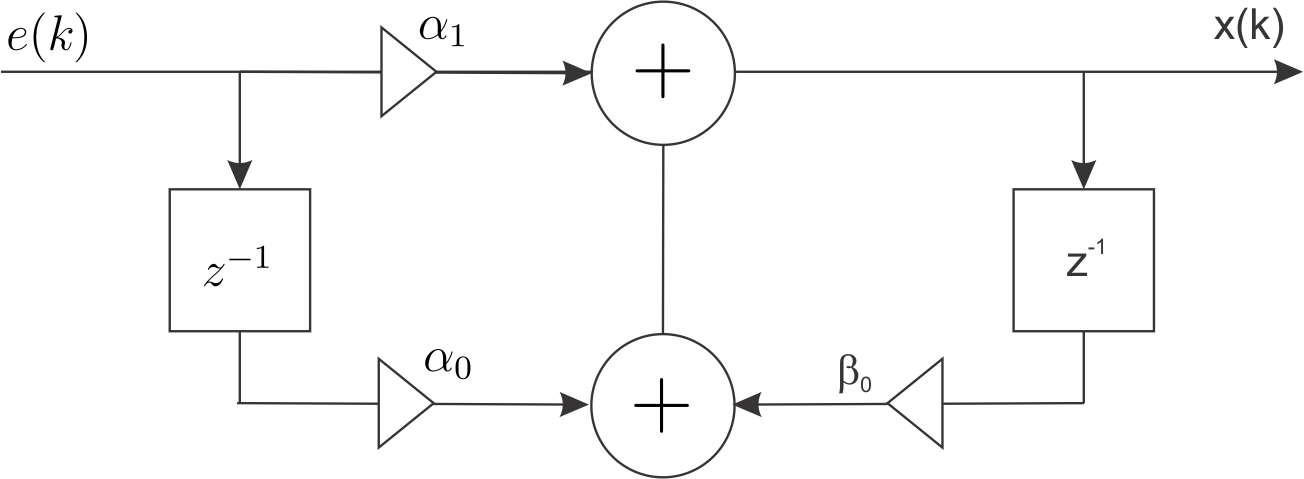
\includegraphics{images/flow2-zzz.png}
\end{center}
\section{Fonts, Emphasis and Shouting}
\label{sec:FontsEmphasisandShouting}

Avoid CAPITALISATION OF WORDS. It is like SHOUTING!

Avoid \underline{underlined words}, unless there it is really necessary.  It is like shouting when normal voice is adequate.

Use emphasis to \textit{emphasise words that must stand out}.
Do not use it too often, perhaps less than three to five times per page. 
Emphasis is like a \textit{waving flag}. If there are \textit{too many flags} waving on a page, it \textit{confuses the reader}.

Use \lstinline{verbatim} to highlight software-related words, such as variable names, module/package/library names, command line text, program output, etc. 
The user associates verbatim font with source code listings, so use verbatim with software `words'.



\section{Math Conventions}
\label{sec:MathConventions}



The IUPAC Green Book, \lstinline{https://en.wikipedia.org/wiki/IUPAC_book}, conveniently summarises international standards in formatting mathematics text and SI units. See also \lstinline{www.tug.org/TUGboat/Articles/tb18-1/tb54becc.pdf} and \lstinline{https://www.iso.org/standard/31887.html}.



The mathematical differential operator must be [ISO 80000-2:2009(E), 2-11.12] upright, not cursive (although pure mathematicians and some house styles prefer cursive).  

\begin{lstlisting}
\usepackage{commath}
\newcommand{\der}{\operatorname{d\!}{}}
$(\der{}x)$  or $(\dif{}x)$ instead of $(dx)$
\end{lstlisting}

\newcommand{\der}{\operatorname{d\!}{}}
$(\der{}x)$  or $(\dif{}x)$ instead of $(dx)$


\begin{lstlisting}
\usepackage{commath}
\begin{equation*}
F(t) = m \od[2]{x(t)}{t}
\end{equation*}
\end{lstlisting}


\begin{equation*}
F(t) = m \od[2]{x(t)}{t}
\end{equation*}


Mathematical variables must be cursive ($\alpha\beta$), but constants must be upright ($\mathrm{\pi}$) not cursive ($\pi$). The code

\begin{lstlisting}
\usepackage[utopia]{mathdesign}
\usepackage[OMLmathrm,OMLmathbf]{isomath}
\newcommand\ct[1]{\text{\rmfamily\upshape #1}}
cursive: $\pi$  $\mathbfit{\pi}$ or upright $\mathrm{\pi}$ $\mathbf{\pi}$\\
or\\
cursive: $e^{i\pi}-1=0$ or upright $\ct{e}^{\ct{i}\piup}-1=0$.
\end{lstlisting}
yields cursive: $\pi$  $\mathbfit{\pi}$ or upright $\mathrm{\pi}$ $\mathbf{\pi}$\\
or \\
cursive: $e^{i\pi}-1=0$ or upright $\ct{e}^{\ct{i}\piup}-1=0$.

Variable subscripts should be typeset in roman if the subscript is a recognisable word:\\
$v_\textrm{aircraft}$ instead of $v_{aircraft}$
\section{Centering in Floats}
\label{sec:CenteringinFloats}

Use \verb=\centering= in floats instead of \verb|\begin{center}\end{center}|, as in 

\begin{verbatim}
\begin{figure}
\centering

\includegraphics[width=0.1\textwidth]{./images/keep-calm-and-code-python_BW.png}
\caption{Keep calm and code Python\label{fig:keep-calm-and-code-python_BW}}
\end{figure}
\end{verbatim}

\section{Forcing Floats to Show}
\label{sec:ForcingFloatstoShow}

The floats accumulate up to a point where some or all of these floats are processed an displayed on a page. The floats are displayed in the order given in the input file.  The rules as to when the float are processed and displayed are not entirely clear to me.  \LaTeX\ appears to have a limit of around 18 unprocessed floats, beyond which an error message is given.  

You can force all unprocessed floats to output in a number of different ways:

\begin{enumerate}
\item
 Use the \verb+\clearpage+ command.  This command immediately stops any further text output and displays all unprocessed floats in the order given.  The problem with this command is that no text is output until all floats are output. This means that if the \verb+\clearpage+ command is near the top of a page, the rest of the page could be empty (unless a float fits there).  

\item
The \verb+\afterpage{}+ command processes whatever command you have given in, after the text on the current page is processed and output. So by using an \verb+\afterpage{\clearpage}+ command at the point where you want to force float output, further text is processed on the current page, filling and outputting  the current page, before the \verb+\clearpage+ command is issued: no more half-empty pages!

\item
The \verb"\FloatBarrier" command causes all unprocessed floats to be processed
immediately. Unlike \verb"\clearpage", it does not start a new page. The command requires the \texttt{placeins} package.

\item
To keep floats in the sections in which they were included, use 
\verb"\usepackage[section]{placeins}".

\item
If you don't want your floats to float, you can use the [H] float specifier from the \verb"float" package. 

\item
If you don't want your figure to float, don't use a floating environment; you can use, for example, a center environment and (if a caption is needed) the \verb"\captionof" command provided by the \texttt{capt-of} (or \texttt{caption}) package.
\lstinline{http://tex.stackexchange.com/questions/32598/force-latex-image-to-appear-in-the-section-in-which-its-declared}


\begin{lstlisting}
\usepackage{capt-of}
\centering
  \includegraphics{foo}
  \captionof{figure}{A non floating figure}
  \label{fig:test}
\end{lstlisting}


\end{enumerate}
\clearpage
\chapter{The ipnb2tex.py Script}
\label{sec:Theipnb2texpyScript}

The \verb+ipnb2tex.py+ reads the IPython notebook and converts it to a \LaTeX{} set of files (a \verb+*.tex+ file and a number of images).  The script is invoked as follows:


\verb+python ipnb2tex.py file.ipynb file.tex imagedir -l+


where


\begin{itemize}
\item \verb+file.ipynb+  [optional]   is the name of the input IPython notebook file.   If no input filename is  supplied, all  \verb+.ipynb+ files in current directory will be processed.   In this event the output filenames will be the same as the \verb+.ipynb+ files, just with a \verb+tex+ filetype.
\item \verb+file.tex+ [optional]  is the name of output \LaTeX{} file. If none is given the output filename will be the same as the input file, but with the \verb+.tex+ extension.
\item \verb+imagedir+   [optional]   is the directory where images are written to.  If not given, this image directory will be the \verb+./pic+ directory.
\item \verb+-i+  [optional], the lower case letter \verb+i+, if this option is given the code     listings are printed inline with the body text where they occur,       otherwise listings are floated to the end of the document.
\item \verb+-u+ [optional] add \verb+\url{}+ to the bibtex entries, to obtain  \verb+url = {\url{http://ipython.org/}}+, otherwise use the form 


\verb+url = {http://ipython.org/}+
\item \verb+--bibstyle=<style>+  [optional] selects bibliography style to be used.
     Use the form 


\verb+--bibstyle=natbib+ or \verb+--bibstyle="natbib"+ [default: \verb+IEEEtran+].
\end{itemize}


\chapter{Heading 1 nb2pdf}
\label{sec:Heading1nb2pdf}

Heading 1 is a \LaTeX{} chapter.


Headings down to level 5 (\LaTeX{} paragraph) are supported. 
Headings at level 6 are treated as normal body text.
If you don't need a chapter (i.e., for an article), just don't use a heading at level 1.


When any level of section heading is formed, a label is automatically created from the text in the heading, removing all non-alpha characters.  If the section heading is very long the the label will also be long, so keep it short. Also, don't use the same text twice as a heading.



\section{Heading 2 Second-level heading}
\label{sec:Heading2Secondlevelheading}


\subsection{Heading 3}
\label{sec:Heading3}


\subsubsection{Heading 4}
\label{sec:Heading4}


\paragraph{Heading 5}
\label{sec:Heading5}


\subparagraph{Heading 6}
\label{sec:Heading6}

some more markdown.



\chapter{Heading 1}
\label{sec:Heading1}


\section{Heading 2}
\label{sec:Heading2}


\subsection{Heading 3}
\label{sec:Heading3}


\subsubsection{Heading 4}
\label{sec:Heading4}


\paragraph{Heading 5}
\label{sec:Heading5}


\subparagraph{Heading 6}
\label{sec:Heading6}


\section{LaTeX Template Format and the Header File}
\label{sec:LaTeXTemplateFormatandtheHeaderFile}


\subsection{Default Style (Report)}
\label{sec:DefaultStyleReport}

The notebook can be converted to the LaTeX \verb+Report+ format with no additional files or document class.  A 'standard' notebook, where the first cell is not \verb+Raw NBConvert+ will be prepended with a short section of LaTeX code for a standard LaTeX Report.  A number of pacakges are also \verb+\usepackage{}+ed, as required by the converted LaTeX code.



\subsection{User-Defined Style}
\label{sec:UserDefinedStyle}

The notebook can optionally be converted to a user-defined format with minimal effort.  The example files included the GitHub distribution provides a 'work package' format class file (\verb+workpackage.cls+) and a header file (\verb+header.tex+).


The first cell of the notebook must be a \verb+RawNBConvert+ cell with at least the following contents (see the first cell of this notebook for an example):


\begin{verbatim}
\documentclass that you want to use
\documentclass{report}

\usepackage{listings}
\usepackage{color}
\usepackage{graphicx}
\usepackage[a4paper, margin=0.75in]{geometry}
\usepackage{textcomp} % additional fonts, required for upquote in listings and \textmu
\usepackage{placeins} % FloatBarrier
\usepackage{url} % for websites
\usepackage[detect-weight]{siunitx} % nice! SI units and print numbers
\usepackage{afterpage} % afterpage{\clearpage}
\usepackage{gensymb} % get the degree symbol as in \celcius
\usepackage{amsmath} 

%the following is required for carriage return symbol
%ftp://ftp.botik.ru/rented/znamensk/CTAN/fonts/mathabx/texinputs/mathabx.dcl
%https://secure.kitserve.org.uk/content/mathabx-font-symbol-redefinition-clash-latex
\DeclareFontFamily{U}{mathb}{\hyphenchar\font45}
\DeclareFontShape{U}{mathb}{m}{n}{
      <5> <6> <7> <8> <9> <10> gen * mathb
      <10.95> mathb10 <12> <14.4> <17.28> <20.74> <24.88> mathb12
      }{}
\DeclareSymbolFont{mathb}{U}{mathb}{m}{n}
\DeclareMathSymbol{\dlsh}{3}{mathb}{"EA}

\usepackage[T1]{fontenc}

\definecolor{LightGrey}{rgb}{0.95,0.95,0.95}
\definecolor{LightRed}{rgb}{1.0,0.9,0.9}

\lstset{ %
upquote=true, % gives the upquote instead of the curly quote
basicstyle=\ttfamily\footnotesize,       % the size of the fonts that are used for the code
numbers=none,                   % where to put the line-numbers
showspaces=false,               % show spaces adding particular underscores
showstringspaces=false,         % underline spaces within strings
showtabs=false,                 % show tabs within strings adding particular underscores
frame=lines,                   % adds a frame around the code
tabsize=4,              % sets default tabsize to 2 spaces
captionpos=b,                   % sets the caption-position to bottom
framesep=1pt,
xleftmargin=0pt,
xrightmargin=0pt,
 captionpos=t,                    % sets the caption-position to top
%deletekeywords={...},            % if you want to delete keywords from the given language
%escapeinside={\%*}{*)},          % if you want to add LaTeX within your code
%escapeinside={\%}{)},          % if you want to add a comment within your code
breaklines=true,        % sets automatic line breaking
breakatwhitespace=false,    % sets if automatic breaks should only happen at whitespace
prebreak=\raisebox{0ex}[0ex][0ex]{$\dlsh$} % add linebreak symbol
}

\lstdefinestyle{incellstyle}{
  backgroundcolor=\color{LightGrey},  % choose the background color,  add \usepackage{color}
  language=Python,
}

\lstdefinestyle{outcellstyle}{
  backgroundcolor=\color{LightRed},   % choose the background color; you must add \usepackage{color} or \usepackage{xcolor}
}

\setlength{\parindent}{0.0mm}
\setlength{\parskip}{6pt}

\begin{document}


whatever preamble lines you require
\begin{document}
\end{verbatim}


Then follows whatever content you need to use your document style, e.g., font style. Write/change this file to change the front  matter and appearance of the document.  The script adds the \verb+\end{document}+ line after the notebook cells' contents.


The \verb+header.tex+ file provides the functionality required by the converter-created code. This content is input using the \LaTeX{} input command.  A number of pacakges are \verb+\usepackage{}+ed, as required by the converted LaTeX code.



\section{Company Logo}
\label{sec:CompanyLogo}

The work package template has a \verb+logo.png+ file which is used to define a logo on top of the page.  The present image is empty, so no logo will show.  You can add your own logo to this file.



\section{The images directory}
\label{sec:Theimagesdirectory}

The script saves the png files in the \verb+./pic+ directory, and the \LaTeX{} code also expects to find the png files there.  Hence, there must be an existing \verb+./pic+ directory in the directory where you run the script.  If an alternative name is given on the command line, the alternative name will be used.



\section{Raw NBConvert cells}
\label{sec:RawNBConvertcells}

The \verb+Raw NBConvert+ cell type can be used to propagate text without any modification to the output stream.  The IPython notebook will not touch this text; it is passed on as-is to the converter code. This this case we can add \LaTeX{} code that will progress straight through to the \LaTeX{} compiler.


This raw capability is very useful if the notebook is intended to be exported to \LaTeX{} as primary output.  I find myself writing most of such documentation in raw latex in a 'Raw NBConvert' cell.  In this mode most of the notebook cells are never rendered to HTML, since you are reading and editing the \LaTeX{} and it stays in \LaTeX{} for display purposes as well. So you get the full benefit of all \LaTeX{} functionality (except that it is not rendered inside the notebook) and all the other benefits of the notebook.


Raw NBConvert cell.  This could be raw \LaTeX{} as in 

\begin{equation}
f_{WN}(\theta;\mu, \sigma) = \frac{1}{\sigma\sqrt{2\pi}}\sum^\infty_{k=-\infty} \exp\left[\frac{-(\theta-\mu+2\pi k)^2}{2\sigma^2}\right]
\end{equation}



\section{Captions}
\label{sec:Captions}

There are three objects that can have captions: listings, figures and tables.


Figures and tables without captions are non-floating and appear in the text at the position it is found in the input file.  Figures and tables with captions are floating.


Listings are always non-floating.


A single cell can contain any combination of captions, and these are indicated in the metadata field of the cell. Select the \verb+Edit Metadata+ drop-down option in the \verb+Cell Toolbar+ drop-down box (towards the right of the toolbar). This should expose metadata buttons on all the cells. Click on the button and type in the  metadata.


The metadata has the following structure:


\begin{verbatim}
{
  "listingCaption": {
    "caption": "Comparison of effective drag parameters",
    "label": "lst:comparedrag",
    "outputCaption": ""
  },
  "figureCaption": {
    "caption": "Caption text for first figure",
    "label": "fig:lab1",
    "width": "0.2",
    "locator": "t"
  },
  "tableCaption": {
    "caption": "Caption text for first table",
    "label": "tab:lab1",
    "format": "{|p{10mm}|l|r|c|c|p{50mm}|p{20mm}|}",
    "fontsize": "normalsize",
    "locator": "t"
  }
}
\end{verbatim}


Note the placement of commas. No newlines are allowed in a single string in the metadata.



\section{Python code}
\label{sec:Pythoncode}

Python code blocks are printed using the \LaTeX{} \verb+listings+ package.  The format details can be defined in the header template file.  These code listings can be supplied with a caption and a label (but these code blocks are not floating entities).


\begin{verbatim}
  {
  "listingCaption": {
    "caption": "Caption text for first listing",
    "label": "lst:listing1",
    "outputCaption": "Caption for first listing output"
  }
}
\end{verbatim}


where the different fields have the following meanings:


\begin{enumerate}
\item \verb+caption+ specifies the text to be used in the listings caption.  If this metadata field is not supplied, the listing will not be given a caption.
\item \verb+label+ specifies the label to be used for the listing, which can be used in \LaTeX{} to reference the listing.  The code block uses the label exactly as given in the metadata field.  If the output listing is given an \verb+outputCaption+, the output caption is labelled by the a label starting with the \verb+label+ string given, but appended with the string \verb+-out+ (i.e., \verb+lst:listing1-out+ in this case).
\item \verb+outputCaption+ specifies the label that is used for the output listing of the cell. If this metadata field is not supplied, the output listing will not be given a caption.
\end{enumerate}

We can refer to Listings~\ref{lst:listing1}, \ref{lst:listing1-out}, \ref{lst:listing2}, and \ref{lst:listing3}.  These listings may not be defined in the IPython output but they are defined in the \LaTeX{} output.


You can also refer to Figures~\ref{fig:lab1-0} and \ref{fig:lab4-2}.


The default is to provide colour syntax highlighting. If you don't want colour in the listings, simply remove these lines from \verb+header.tex+


\begin{verbatim}
commentstyle=\color{mygreen},    \% comment style
keywordstyle=\color{blue},       \% keyword style
stringstyle=\color{mymauve},     \% string literal style
\end{verbatim}



\section{Floated code listings}
\label{sec:Floatedcodelistings}

In order to improve readability in the document, the code listings can be floated to the end of the document by using the \verb+-l+ switch on the command line.  If this switch is used, the listing is saved to a string that is only appended to the \LaTeX{} document and the end of the conversion.  At the location in the document where the code listing would have been, a reference sentence to the code is included.  The  sentence is constructed as follows:


\verb+See Listing~\ref{lst:autolistingcellX} for the code {purpose}.+


where the symbolic link is constructed using the cell number and the text used in the \verb+{purpose}+ part is taken from the first line of the code, if the first line is a comment with a single \verb+#+ followed by a space.  Hence if the code in cell 3 starts with the lines


\begin{verbatim}
# to prepare the environment
import numpy as np
\end{verbatim}


a text line of the following form will be created:


\verb+See Listing~\ref{lst:autolistingcell3} for the code to prepare the environment.+


Just maintain the discipline to write good comments in the first line, keeping in mind that  the comment will end up in the body of the document with the reference.


If a code cell does not start with a comment, no text will be inserted and the form will be


\verb+See Listing~\ref{lst:autolistingcell24} for the code.+


If the code cell starts with a comment of the form \verb+##+, the listing will output to the tex file, but there is no text entry in the location where the code cell was. i.e., no line starting with \verb+See Listing+...


If the code cell starts with a comment of the form \verb+###+, neither the listing nor the  text entry referring to it is written to the latex file.  So if you don't want the code to be shown or a reference to it made, start the first code line with \verb+###+.




See Listing~\ref{lst:listing1} for the code  to prepare the environment.


\begin{lstlisting}[style=outcellstyle,caption={Caption for first listing output \label{lst:listing1-out}}]
The Zen of Python, by Tim Peters

Beautiful is better than ugly.
Explicit is better than implicit.
Simple is better than complex.
Complex is better than complicated.
Flat is better than nested.
Sparse is better than dense.
Readability counts.
Special cases aren't special enough to break the rules.
Although practicality beats purity.
Errors should never pass silently.
Unless explicitly silenced.
In the face of ambiguity, refuse the temptation to guess.
There should be one-- and preferably only one --obvious way to do it.
Although that way may not be obvious at first unless you're Dutch.
Now is better than never.
Although never is often better than *right* now.
If the implementation is hard to explain, it's a bad idea.
If the implementation is easy to explain, it may be a good idea.
Namespaces are one honking great idea -- let's do more of those!

\end{lstlisting}

The following code block has the metadata


\begin{verbatim}
{
  "listingCaption": {
    "caption": "Caption text for second listing",
    "label": "lst:listing2"
  }
}
\end{verbatim}


which will give the code block a caption and a label, but the output is not captioned.


The code block also demonstrates how long lines are handled in this lstlistings configuration, with a linefeed symbol to mark the line.



\begin{lstlisting}[style=outcellstyle]
 
Radius = 6
Frontal area = 7 m2
This is a very long line of python code, that is supposed to flow over to the next line, in order to test the listing display

\end{lstlisting}



See Listing~\ref{lst:listing3} for the code  to print the value.


\begin{lstlisting}[style=outcellstyle]
a
b

\end{lstlisting}


\begin{lstlisting}[style=outcellstyle]
0
1

\end{lstlisting}

The following code block has no metadata, and hence no captions on either the code or the output listings.




See Listing~\ref{lst:autolistingcell64} for the code.


\begin{lstlisting}[style=outcellstyle]
code with no listing caption

\end{lstlisting}

Output emanating from different cells \textit{may} result in different output listings in \LaTeX{} even if they appear in a single output box in the notebook.  The cells below attempt to recreate a similar scenario in a different application, but it does not seem to repeat the problem here.




See Listing~\ref{lst:autolistingcell66} for the code.



See Listing~\ref{lst:autolistingcell67} for the code.


\begin{lstlisting}[style=outcellstyle]
function output 1
function output 2
function output 3
9
3

\end{lstlisting}


\section{Bitmaps}
\label{sec:Bitmaps}

PNG images, read in from externally or created by Matplotlib, are imported into the \LaTeX{} code with lines of the following form:


\verb+\includegraphics[width=WIDTH\textwidth]{./pngs/test2LaTeX\_21\_0.png}+


where the WIDTH determines the size of the image (obtained from metadata, see below), and the image file name is constructed from the notebook file name and cell information.  The name is the concatenation of the notebook file name, the cell index (index number of the cell in the notebook file) and the sub-index image in the cell's output (there can be more than one image). All indices are zero based.


The width is read from the metadata, which must be structured as follows:


\begin{verbatim}
{
  "figureCaption": {
    "caption": "Caption text for first figure",
    "label": "fig:lab1",
    "width": "0.2",
    "locator": "t"
  },
  "listingCaption": {
    "caption": "Listing caption in cell with a figure",
    "label": "lst:figurelisting",
    "outputCaption": "Output for a cell with a figure"
  }
}
\end{verbatim}


Width is the fraction of \LaTeX{} textwidth, i.e., if width=1, the graphic will be the full width of the text on the page.


The locator value is used in \verb+\begin{figure}[tb]+ or \verb+\begin{table}[tb]+ to locate the float on the page. Default value is 'tb', can be any combination of \verb+tbhp+.


The metadata also contains a caption string, and a label for the figure.  The type must be \verb+figure+.


If the \verb+caption+ field is given (or has non-zero length), the image will be written to a \LaTeX{} float with a caption (and label).  If the \verb+caption+ fields is not given, the image will not be encapsulated in the floating figure.


To edit the meta data: on the left panel click on the Property Inspector (gear icon) and open the \verb+Advanced Tools+ drop-down to expose the \verb+Cell Metadata+ text box.
Enter the meta data into the text box. Ensure that the tabs and commas are all in the right places: if so, a small tick mark will appear for you to approve the new metadata, by clicking on the tick mark.  If the tabs and commas are not exactly right, the text box boundary will be red (error) and the tick mark will not be shown.




See Listing~\ref{lst:figurelisting} for the code this figure is given meta data caption parameters, it will be floated in the latex export.


\begin{figure}[tb]
\centering
\includegraphics[width=0.2\textwidth]{./pic/test2LaTeX_71_0.png}
\caption{Caption text for first figure\label{fig:lab1-0}}
\end{figure}


\begin{lstlisting}[style=outcellstyle,caption={Output for a cell with a figure \label{lst:figurelisting-out}}]
also force print output

\end{lstlisting}

Experimenting with embedded markdown images:


\begin{center}

\includegraphics[width=0.9\textwidth]{images/keep-calm-and-code-python_BW.png}
\end{center}


The following figure is not floating, but with narrower width.


\begin{verbatim}
{
  "figureCaption": {
    "width": "0.3"
  }
}
\end{verbatim}




See Listing~\ref{lst:autolistingcell74} for the code this figure is not given meta data caption parameters, it will be inlined in the latex export.

\begin{center}
\includegraphics[width=0.3\textwidth]{./pic/test2LaTeX_74_0.png}
\end{center}

The following Matplotlib plot is scaled to 40\% of text width and floating, but with the 'h' locator to force the location to here.


\begin{verbatim}
{
  "figureCaption": {
    "caption": "Caption text for third figure",
    "label": "fig:lab3",
    "width": "0.4",
    "locator": "h"
  }
}
\end{verbatim}




See Listing~\ref{lst:autolistingcell76} for the code.


\begin{figure}[h]
\centering
\includegraphics[width=0.4\textwidth]{./pic/test2LaTeX_76_0.png}
\caption{Caption text for third figure\label{fig:lab3-0}}
\end{figure}

It is possible to have more than one plot in a single cell output.  In this case each output can be made floating separately or be non-floated (you can even mix floating and non-floating).  The captions are given in the metadata in the following format:


\begin{verbatim}
{
  "figureCaption": {
    "caption": "['Caption text for (first) fourth figure','','Caption text for (third) fourth figure']",
    "label": "fig:lab4",
    "width": "[0.5, 0.5, 0.5]"
  }
}
\end{verbatim}


In this case the caption strings and scaling values are allocated to the sequence of images in the order given.  If a caption string is zero length, that specific image will be non-floating.  The float labels are determined from the root value given in the metadata, but with the output sub-index appended, as in \verb+fig:lab4-0+, \verb+fig:lab4-1+, \verb+fig:lab4-2+.




See Listing~\ref{lst:autolistingcell78} for the code.


\begin{figure}[tb]
\centering
\includegraphics[width=0.5\textwidth]{./pic/test2LaTeX_78_0.png}
\caption{Caption text for (first) fourth figure\label{fig:lab4-0}}
\end{figure}

\begin{center}
\includegraphics[width=0.5\textwidth]{./pic/test2LaTeX_78_1.png}
\end{center}


\begin{figure}[tb]
\centering
\includegraphics[width=0.5\textwidth]{./pic/test2LaTeX_78_2.png}
\caption{Caption text for (third) fourth figure\label{fig:lab4-2}}
\end{figure}

\FloatBarrier % message to latex, no floats past this barrier
You can write HTML to the cell's output and have it displayed in the browser and also in the LaTeX file.




See Listing~\ref{lst:autolistingcell81} for the code.

\begin{center}
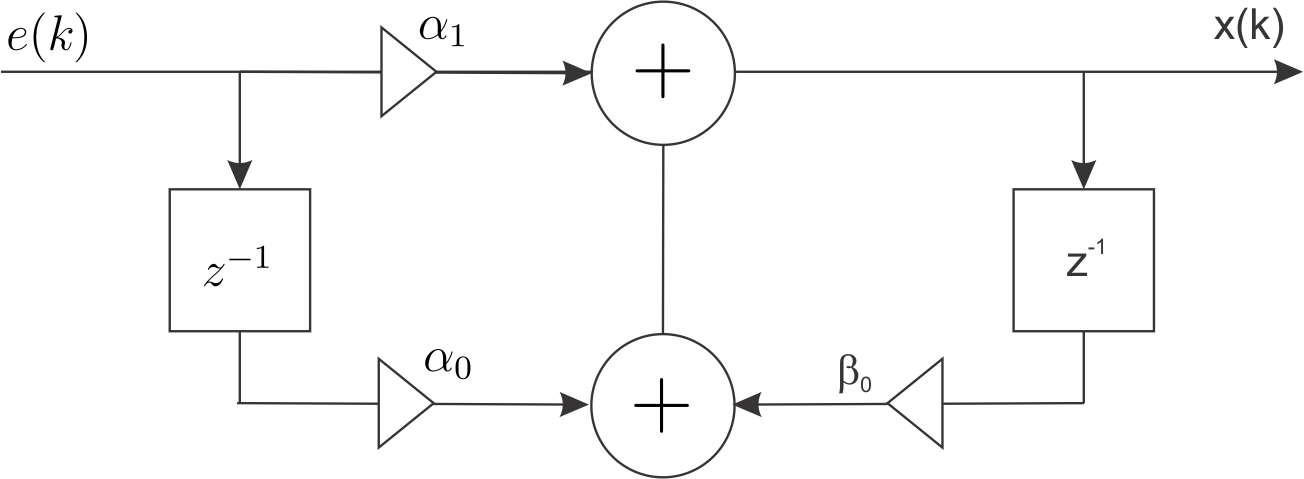
\includegraphics[width=0.9\textwidth]{images/flow2-zzz.png}
\end{center}


There might be a picture before this text if the HTML pictures are exporting :-)


Experimenting with embedded markdown images. The figures should be 
Figure~\ref{fig:keepcalm-0} and 
Figure~\ref{fig:keepcalm-1}.


{

\begin{figure}[t]
\centering

\includegraphics[width=0.1\textwidth]{images/keep-calm-and-code-python_BW.png}
\caption{Keep calm 1\label{fig:keepcalm-0}}
\end{figure}

}


{

\begin{figure}[t]
\centering
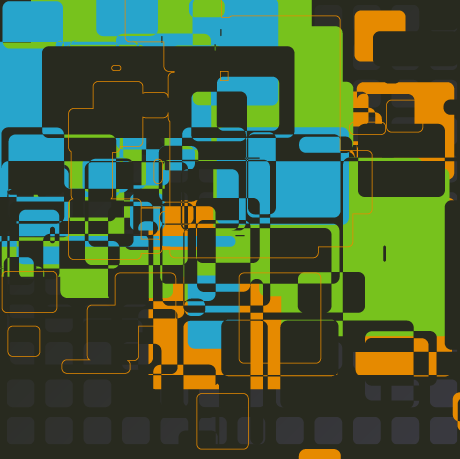
\includegraphics[width=0.2\textwidth]{images/random-squares-2.png}
\caption{Keep calm 2\label{fig:keepcalm-1}}
\end{figure}

}



\section{Graphs as PDF documents}
\label{sec:GraphsasPDFdocuments}

Reports with many png images tends to create large PDF files.    If the graphs are exported as PDF files by the backend, the files are vector graphics and not large bitmaps, resulting in a much smaller final PDF report file.


The PDF export functionality worked well in brief testing, but it still needs more testing.


\begin{enumerate}
\item Set up the notebook to use the PDF backend:
        \%config InlineBackend.figure\_format = 'pdf'
\item With the PDF backend the graphs are saved as PDF documents in the notebook.  This converter script will export these as PDF files to the pictures directory.
\item Compile the document with PDFLaTeX as usual.  It will look for the graphics files as PDF files, not PNG files.
\end{enumerate}


\section{Cells with Python errors}
\label{sec:CellswithPythonerrors}

The following line must be uncommented to have effect.




See Listing~\ref{lst:autolistingcell88} for the code  type(eval("this is a test string")) is not list.


\section{Embedded code (verbatim text)}
\label{sec:Embeddedcodeverbatimtext}

Some firewalls are set up to grant \verb+localhost+ execution rights.  In this case the server can be started with the command


\verb+ipython notebook --ip=localhost+


Once started, the pages are served from 


\verb+http://localhost:8888/+


and not from \verb+http://127.0.0.1:8888/+.


Embedded code meant for illustration instead of execution in Python:


\begin{verbatim}
def hello\_ipython():
    print "Hello IPython!"
\end{verbatim}



\section{Hyperlinks, references and citations}
\label{sec:Hyperlinksreferencesandcitations}


\subsection{Embedded hyperlinks}
\label{sec:Embeddedhyperlinks}

The IPython website\cite{httpipythonorg} is the central repository of all things IPython.
There are some really nice videos\cite{httpswwwyoutubecomwa00000} on YouTube.


For \textit{URI references}, the \verb+[IPython website](http://ipython.org/)+ markup structure is read and the URI is used to create a citation label (\verb+httpipythonorg+) and the URI (\verb+http://ipython.org/+) is written to a new \LaTeX{} bibtex file for the references in this notebook.


For \textit{other types of references} a workaround is required.  IPython is currently weak in the area of other types of references, because of limitations in the markup language.  The \verb+ipnb2tex.py+ script makes provision for including bibtex entries, by embedding the complete bibtex entry in a metadata field.


Using the above approach creates a new bibtex file using the data in the notebook. Perhaps you might want to reference an existing bibtex file, mapping to the citation labels used in the notebook.
The issue here is that the IPython notebook does not have access to your \LaTeX{} bibtex file, so it does not know the citation references you want to use (the ones in your existing bibtex file).


The approach taken here is to provide a look-up translation table in this or any prior cell of the notebook, to translate citation references from the local name to your existing bibtex name.  This is done in a cross reference dictionary that maps the names created internally to the names in your external bibtex file.


The metadata has two different fields, one to do the citation label mapping and the other to embed complete bibtex entries in the metadata.  The metadata field must have the following format:


\begin{verbatim}
{
  "bibxref": {
    "httpipythonorg": "httpipythonorg",
    "httpswwwyoutubecomwatchvaIXED26Wppg": "httpswwwyoutubecomwatchvaIXED26Wppg",
    "httpsenwikipediaorgwikiWrappednormaldistribution": 
            "httpsenwikipediaorgwikiWrappednormaldistribution"
  },
  "bibtexentry": {
    "wing2006computational": "@article{wing2006computational,  title={Computational thinking},  
           author={Wing, Jeannette M},  journal={Communications of the ACM},  volume={49},  
           number={3},  pages={33--35},  year={2006}}",
    "gracec": "@MISC{gracec,  author = {Grace Cathedral},  title = {The Cathedral Labyrinths},  
           url = {http://www.gracecathedral.org/labyrinth/}}"
  }
}
\end{verbatim}


where (1) the bibxref keys are the local names and the values are the names in your existing bibtex file and (2) the bibtexentry keys are the citation labels used in the notebook.  In the above example the bibxref maps to the same names, because I am using the locally generated bibtex file. Normally you would use your bibtex database entries.


Note that the IPython notebook is somewhat finicky on the json format; each single entry in the above metadata must be on a single line (line-feeds inside the strings are not allowed --- lines tend to be very long).  Also, note the location of commas, there should be commas after all entries, except the last entry in a given scope.


The \verb+ipnb2tex.py+ script:


\begin{enumerate}
\item Loads/appends the bibxref translation table from any/all cells (if present).
\item Reads the \verb+[]()+ markup structure and then builds a citation reference from the URI (by removing some characters).
\item Create a bibtex entry for the reference (subsequently written to file).
\item Using bibxref, translates the local citation label to your existing citation label.
\end{enumerate}

If you included bibtex items in the metadata, you can refer to them using the normal \LaTeX{} notation. Test \cite{wing2006computational} and \cite{gracec}.


At the conclusion of the processing the script reads all existing \verb+*.bib+ files in the cirrent folder and combine all of them into one file.  This way you can include prior existing bib files.



\section{General markdown formatting}
\label{sec:Generalmarkdownformatting}

Markdown basics: lists, markup and code


\begin{itemize}
\item list item1   in markdown format.
\item list item2   \begin{itemize}
\item nested list item3 - font attributes not yet supported.
\end{itemize}
\item \textit{italics}
\item \textbf{bold}
\item \verb+fixed font+
\end{itemize}




\begin{enumerate}
\item Enumerated list item 1 in markdown format.\begin{enumerate}
\item sub lit element 1
\item sub lit element 2
\end{enumerate}
\item Enumerated list item 2.
\end{enumerate}

The markup language (or the converter) breaks if an itemized list and an enumerated list are immediately adjacent --- we need to separate the lists by text with with a \verb+<p/>+.


Please note that the converter does not currently allow free standing (enter-twice) paragraphs inside lists.  Please make the paragraphs touch and use double spaces at the end to force a new line. This will be converted to loose standing paragraphs in LaTeX.


\begin{enumerate}
\item list item1 in markdown format.
\item list item2  


   item2 new parra 1 


   item2 new parra 1
\item list item3


    item3 new parra 1


    item3 new parra 2
\item list item4 [ this does not work correctly ]


list item4 [ this does not work correctly ]


item4 new parra 1 [ this does not work correctly ]


list item4 [ this does not work correctly ]


list item4 [ this does not work correctly ]


item4 new parra 1 [ this does not work correctly ]


item4 new parra 2 [ this does not work correctly ]
\item list item5  [ this should work correctly ]   


     item5 new parra 1    [ this should work correctly ]. We reference Figure~\ref{fig:propflightpaths-0} here.   


{

\begin{figure}[t]
\centering
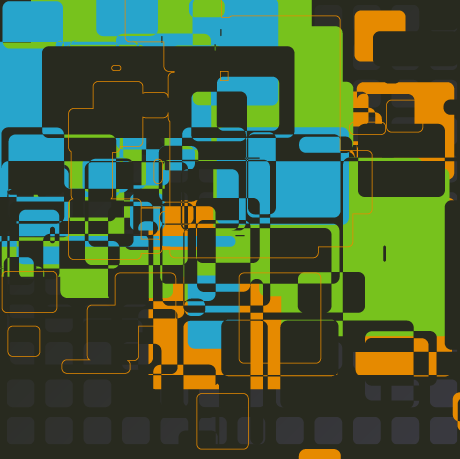
\includegraphics[width=0.1\textwidth]{images/random-squares-2.png}
\caption{Proposed flight paths\label{fig:propflightpaths-0}}
\end{figure}

}




     item5 new parra 2    [ this should work correctly ]
\end{enumerate}

Lists in HTML format


\begin{itemize}
\item list item
\item list item
\begin{itemize}
\item nested list item
\end{itemize}
\item \textit{italics}
\item \textbf{bold}
\item \verb+fixed font+
\end{itemize}

\begin{enumerate}
\item Enumerated list item 1.
\begin{enumerate}
\item sub lit element 1
\item sub lit element 2
\end{enumerate}
\item Enumerated list item 2.
\end{enumerate}


\section{Tables}
\label{sec:Tables}

The table in this cell is rendered in \LaTeX{} with the following metadata:


\begin{verbatim}
{
  "tableCaption": {
    "caption": "Caption text for first table",
    "label": "tab:lab1",
    "format": "{|p{10mm}|l|r|c|c|p{50mm}|p{20mm}|}",
    "fontsize": "normalsize",
    "locator": "t"
  }
}
\end{verbatim}


A complex HTML table with row spans and column spans:



\begin{table}[tb]
\centering
\caption{Caption text for first table\label{tab:lab1-0}}

\begin{normalsize}

\begin{tabular}{{|p{10mm}|l|r|c|c|p{50mm}|p{20mm}|}}
\hline
a&\multicolumn{2}{|c|}{b}&\multicolumn{3}{|c|}{c}&1\\\hline
e&f&\multicolumn{2}{|c|}{g}&h&i&2\\\cline{2-2}\cline{3-3}\cline{4-4}\cline{5-5}\cline{6-6}\cline{7-7}
&\multicolumn{2}{|c|}{j}&k&l&m&3\\\cline{1-1}\cline{2-2}\cline{3-3}\cline{4-4}\cline{6-6}\cline{7-7}
n&o&p&q&&r&4\\\hline
s&t&u&v&w&x&5\\\hline

\end{tabular}
\end{normalsize}
\end{table}

The tables in this cell are rendered in \LaTeX{} with the following metadata:


\begin{verbatim}
{
  "tableCaption": {
    "caption": "['Caption text for (first) second table','','Caption text for (third) second table']",
    "label": "tab:lab2",
    "format": "['{|p{20mm}|r|}','','{|c|l|}']",
    "fontsize": "['normalsize', 'tiny', 'Large']"
  }
}
\end{verbatim}


Github flavoured markdown tables are supported in the IPython notebook (floating in \LaTeX{} as Table~\ref{tab:lab2-0}):



\begin{table}[tb]
\centering
\caption{Caption text for (first) second table\label{tab:lab2-0}}

\begin{normalsize}

\begin{tabular}{{|p{20mm}|r|}}
\hline
This&is\\\hline
a&table\\\hline

\end{tabular}
\end{normalsize}
\end{table}

second table  (non-floating in \LaTeX{}):



\begin{table}[tb]
\centering
\caption{Caption text for (third) second table\label{tab:lab2-2}}

\begin{Large}

\begin{tabular}{{|c|l|}}
\hline
This&is\\\hline
a&small table\\\hline

\end{tabular}
\end{Large}
\end{table}

PHP Markdown Extra is also supported  (floating in \LaTeX{} as Table~\ref{tab:lab2-2}):


\begin{center}

\begin{normalsize}

\begin{tabular}{|c|c|}
\hline
First Header&Second Header\\\hline
Content Cell&Content Cell\\\hline
Content Cell&Content Cell\\\hline

\end{tabular}
\end{normalsize}
\end{center}

Both of these markup extensions require Python Markdown 2.4.1 to render HTML.


Table~\ref{tab:hiertab12-0} has an hierarchical structure on both columns and rows.  The percentage and underline characters are also preserved.

\begin{table}[tb]
\centering
\caption{Caption text for hierarchical table\label{tab:hiertab12-0}}

\begin{normalsize}

\begin{tabular}{|l|l|l|*{2}{>{\RaggedLeft}p{8mm}|}}
\hline
&&CHead 1&\multicolumn{2}{|c|}{CLevel 1:1}\\\hline
&&CHead 2&CLevel 2:1&CLevel 2:2\\\hline
RHead 1&RHead 2&RHead 3&&\\\hline
RLevel 1:1\%\_&RLevel 2:1&A&6000\%&6156\\\cline{3-3}\cline{4-4}\cline{5-5}
&&B&2417&2471\\\cline{3-3}\cline{4-4}\cline{5-5}
&&C&1274&1347\\\cline{2-2}\cline{3-3}\cline{4-4}\cline{5-5}
&RLevel 2:2&A&10909&11041\\\cline{3-3}\cline{4-4}\cline{5-5}
&&B&4400&4408\\\cline{3-3}\cline{4-4}\cline{5-5}
&&C&2309&2319\\\cline{2-2}\cline{3-3}\cline{4-4}\cline{5-5}
&RLevel 2:3&A&11573&11178\\\cline{3-3}\cline{4-4}\cline{5-5}
&&B&4461&4976\\\cline{3-3}\cline{4-4}\cline{5-5}
&&C&2432&2410\\\hline
RLevel 1:2\%\_&RLevel 2:1&A&6728&6595\\\cline{3-3}\cline{4-4}\cline{5-5}
&&B&2322&2679\\\cline{3-3}\cline{4-4}\cline{5-5}
&&C&1300&1474\\\cline{2-2}\cline{3-3}\cline{4-4}\cline{5-5}
&RLevel 2:2&A&1210&12344\\\cline{3-3}\cline{4-4}\cline{5-5}
&&B&4845&4367\\\cline{3-3}\cline{4-4}\cline{5-5}
&&C&2618&2525\\\cline{2-2}\cline{3-3}\cline{4-4}\cline{5-5}
&RLevel 2:3&A&12553&12117\\\cline{3-3}\cline{4-4}\cline{5-5}
&&B&4895&4835\\\cline{3-3}\cline{4-4}\cline{5-5}
&&C&2566&2991\\\hline

\end{tabular}
\end{normalsize}
\end{table}

The infrared sensor example has the following design characteristics:


\begin{center}

\begin{normalsize}

\begin{tabular}{|c|c|c|c|}
\hline
Characteristic&Value&Unit&Motivation\\\hline
Spectral response&3.7--4.9&$\mu$m&detector specification\\\hline
Pixel size (x and y)&12&$\mu$m&detector specification\\\hline
Pixel fill factor&0.95&&detector specification\\\hline
Detector temperature&80&K&detector specification\\\hline
Detector external quantum efficiency&0.8&&detector specification\\\hline
Detector internal quantum efficiency&0.75&&detector specification\\\hline
Number rows&144&-&detector specification\\\hline
Number columns&256&-&detector specification\\\hline
Detector PRNU  stddev&0.2&&detector specification\\\hline
Well capacity at 1 V&$3.2\times 10^{6}$&e&detector specification\\\hline
Sense node voltage&3.0 $\rightarrow$ 1.0&V&detector specification\\\hline
F-number&3.2&-&detector specification\\\hline
Band gap 0~K&0.235&eV&material property\\\hline
Varshni A&0.00068&&material model\\\hline
Varshni B&500&&material model\\\hline
Dark FOM&$4\times 10^{-9}$&nA/cm$^2$&material model\\\hline
Dark cm&1&&material model\\\hline
Dark FPN stddev&0.4&&material model\\\hline
Well capacitance at 1.0 V&$5.13\times 10^{-13}$&F&by calculation\\\hline
k1&$5.13\times 10^{-13}$&CV&by calculation\\\hline
Gain at 1.0 V&$3.125\times 10^{-7}$&V/e&by calculation\\\hline
Pixel IFOV (x and y)&$100.0\times 10^{-6}$&rad&design choice\\\hline
Frame time&0.02&s&design choice\\\hline
Focal length&0.12&m&design choice\\\hline
Full field angle&0.84&deg&focal length and detector\\\hline

\end{tabular}
\end{normalsize}
\end{center}

Charge well (sense node) capacitance $C = nq/V$. The charge well is filled to capacity at the minimum sense node voltage $C = \num{3.2e6}\times\num{1.6e-19}/1.0= \num{0.513e-12}$~F.  Then $k_1=CV=\num{0.513e-12}\times 1=\num{0.513e-12}$.


Sense node gain is given by $V/n = q/C = \num{1.6e-19}/\num{0.513e-12}=\num{3.12e-07}$ V/e.


A table can be formatted with the metadata, even if the table is not floating with a caption. For example, the following table only uses the following metadata:


\begin{verbatim}
{
  "tableCaption": {
    "format": "{|p{10mm}|p{50mm}|p{100mm}|}",
    "fontsize": "footnotesize"
  }
}
\end{verbatim}


\begin{center}

\begin{footnotesize}

\begin{tabular}{{|p{10mm}|p{50mm}|p{100mm}|}}
\hline
Column Number&Column Description&Example Values\\\hline
1&Unique row identifier&MOD15A2.A2000057.h12v03.004.2002357024124.FparExtra\_QC
        MOD15A2.A2000057.h12v03.004.2002357024124.Lai\_1km\\\hline
2&MODIS Land Product 
        Code&MOD15A2\\\hline
3&MODIS Acquisition 
        Date [ A (YYYYDDD) ]&A2000057\\\hline
4&User selected center 
        point coordinates and specified width (Samp) and height (Line) of 
        bounding rectangle in pixels. Width x height denotes number of 
        Product values starting in Column 7. (e.g.,  7 x 7 $=$ 49)&Lat55.879620Lon-98.480810Samp7Line7\\\hline
5&MODIS Processing Date 
        (YYYYDDDHHMMSS)&2002357024124\\\hline
6&Product Scientific 
        Data Set (Band): Indicates type of values to follow. Specific values 
        vary by Product. Data quality information are interleaved.&MOD15A2: FparExtra\_QC,  
        FparLai\_QC,  Fpar\_1kmMOD17A2: Gpp\_1km,  PsnNet\_1km,  Psn\_QC\_1km\\\hline
7 to N&Data values of type 
        as specified. Number of data columns as given in Column 4.
        Definition of QC component values vary by Scientific Data Set.&QC: 
        00100001, 01100001, 01100001,  ...Measurement: 
        2, 2, 1, 1, 1, 1, 1, 0, 0, 0, 1, 1, 0, 0, ...to N\\\hline

\end{tabular}
\end{footnotesize}
\end{center}

Pandas dataframe tables are also rendered.




See Listing~\ref{lst:autolistingcell104} for the code.

\begin{center}

\begin{normalsize}

\begin{tabular}{|c|c|c|}
\hline
&one&two\\\hline
a&1.0&1.0\\\hline
b&2.0&2.0\\\hline
c&3.0&3.0\\\hline
d&NaN&4.0\\\hline

\end{tabular}
\end{normalsize}
\end{center}


\chapter{Embedding LaTeX code in output cells}
\label{sec:EmbeddingLaTeXcodeinoutputcells}

Jupyer uses MathJax for LaTeX rendering in the markdown cells.  This is very useful for documentation in general, but sometimes MathJax is not sufficient for special LaTeX constructs. LaTeX constructs can be embedded (but not rendered in Jupyter) in output cells.   The LaTeX in the output cell can then be rendered/typeset when the converted LaTeX document is built.


Any string you construct in a code cell and then use the \verb+IPython.display.Latex+ function to display will be embedded in the output cell as a data of mime type \verb+text/latex+.  The ipynb2tex converter will then process this LaTeX in the output cell as regular LaTeX in the target document.  So the following code:


\begin{verbatim}
from IPython.display import Latex
lstr = 'This is a \LaTeX string.'
Latex(lstr)
\end{verbatim}


Will make a mime type \verb+text/latex+ data entry with the contents of \verb+lstr+ in the output cell.  When rendered in the notebook, it will simply show the text as entered.


With this functionality, LaTeX code of any complexity can be constructed by code, for eventual typesetting by the LaTeX compiler after the notebook has been converted to LaTeX.



\section{Pandas DataFrame to LaTeX}
\label{sec:PandasDataFrametoLaTeX}

The following example shows how to export a Pandas dataframe to a \verb+IPython.core.display.Latex object+ in the string \verb+lstr+. When viewed in the notebook, the table is shown as a LaTeX code, but when the conversion to a LaTeX document takes place, the LaTeX is rendered as regular LaTeX in the output PDF file.


The table format specification is provided by the Pandas  to\_latex(column\_format)\cite{httppandaspydataorgp00001} argument,  as in


\verb+'|l|l|p{50mm}|c|r|'+




See Listing~\ref{lst:autolistingcell108} for the code  to create the dataframe and write the output to LaTeX object at default font size.

{
\renewcommand{\arraystretch}{1.1}
\centering
% to get unbroken vertical lines with booktabs, set separators to zero
% also set all horizontal lines to same width
\aboverulesep=0ex
\belowrulesep=0ex
\heavyrulewidth=.05em
\lightrulewidth=.05em
\cmidrulewidth=.05em
\belowbottomsep=0pt
\abovetopsep=0pt

\begin{normalsize}
\begin{tabular}{|l|l|p{50mm}|c|r|}
\toprule
{} &         A &         B &         C &         D \\
\midrule
2013-01-01 & -0.471166 & -1.037291 & -0.537825 & -0.769806 \\
2013-01-02 &  1.482872 & -0.486803 & -1.549107 &  1.261904 \\
2013-01-03 & -0.807543 & -1.421014 &  0.348899 &  0.151206 \\
2013-01-04 & -0.944017 &  1.432089 &  1.527693 & -0.088178 \\
2013-01-05 & -0.739531 & -0.568235 & -0.709687 & -0.104466 \\
2013-01-06 & -1.217844 &  1.522592 & -0.869592 &  1.010980 \\
\bottomrule
\end{tabular}

\end{normalsize}
\renewcommand{\arraystretch}{1}
}



See Listing~\ref{lst:autolistingcell109} for the code.

{
\renewcommand{\arraystretch}{1.1}
\centering
% to get unbroken vertical lines with booktabs, set separators to zero
% also set all horizontal lines to same width
\aboverulesep=0ex
\belowrulesep=0ex
\heavyrulewidth=.05em
\lightrulewidth=.05em
\cmidrulewidth=.05em
\belowbottomsep=0pt
\abovetopsep=0pt

\begin{normalsize}
\begin{tabular}{|l|l|p{50mm}|c|r|}
\toprule
        A &         B &         C &         D \\
\midrule
-0.471166 & -1.037291 & -0.537825 & -0.769806 \\
 1.482872 & -0.486803 & -1.549107 &  1.261904 \\
-0.807543 & -1.421014 &  0.348899 &  0.151206 \\
-0.944017 &  1.432089 &  1.527693 & -0.088178 \\
-0.739531 & -0.568235 & -0.709687 & -0.104466 \\
-1.217844 &  1.522592 & -0.869592 &  1.010980 \\
\bottomrule
\end{tabular}

\end{normalsize}
\renewcommand{\arraystretch}{1}
}

Set the font size for the typesetting by using the \verb+latex/fontsize+ setting in the  cell json metadata.
Use the regular LaTeX font size definitions but without the backslash (Huge, huge, LARGE, Large, large, normalsize, small, footnotesize, scriptsize, tiny):


\begin{verbatim}
{
  "latex": {
    "fontsize": "LARGE"
  }
}
\end{verbatim}


Of course you may have to use this setting in conjunction with any other json settings.




See Listing~\ref{lst:autolistingcell111} for the code  to write the table in LARGE.

{
\renewcommand{\arraystretch}{1.1}
\centering
% to get unbroken vertical lines with booktabs, set separators to zero
% also set all horizontal lines to same width
\aboverulesep=0ex
\belowrulesep=0ex
\heavyrulewidth=.05em
\lightrulewidth=.05em
\cmidrulewidth=.05em
\belowbottomsep=0pt
\abovetopsep=0pt

\begin{LARGE}
\begin{tabular}{|l|l|p{50mm}|c|r|}
\toprule
{} &         A &         B &         C &         D \\
\midrule
2013-01-01 & -0.471166 & -1.037291 & -0.537825 & -0.769806 \\
2013-01-02 &  1.482872 & -0.486803 & -1.549107 &  1.261904 \\
2013-01-03 & -0.807543 & -1.421014 &  0.348899 &  0.151206 \\
2013-01-04 & -0.944017 &  1.432089 &  1.527693 & -0.088178 \\
2013-01-05 & -0.739531 & -0.568235 & -0.709687 & -0.104466 \\
2013-01-06 & -1.217844 &  1.522592 & -0.869592 &  1.010980 \\
\bottomrule
\end{tabular}

\end{LARGE}
\renewcommand{\arraystretch}{1}
}

An exported \verb+IPython.core.display.Latex object+ Pandas dataframe can also be typeset as a floating table by setting appropriate metadata for the floating table:


\begin{verbatim}
{
  "latex": {
    "fontsize": "scriptsize"
  },
  "tableCaption": {
    "caption": "Caption text for Pandas table",
    "label": "tab:lab1",
    "format": "IGNORED!!",
    "fontsize": "tiny"
  }
}
\end{verbatim}


If both \verb+latex/fontsize+ and \verb+tableCaption/fontsize+ are present then the \verb+tableCaption/fontsize+ takes preference, and the table (only) is rendered in the specified fontsize.  The floating caption is in the normal document font size.


The table format specification is provided by the Pandas \verb+.to\_latex(column\_format)+  argument, so the \verb+tableCaption/format+ specification in the json is ignored.




See Listing~\ref{lst:autolistingcell113} for the code  to write a floating table in tiny font size.

{

\begin{table}[tb]
\centering
\caption{Caption text for the Pandas table\label{tab:lab1-0}}
% to get unbroken vertical lines with booktabs, set separators to zero
% also set all horizontal lines to same width
\aboverulesep=0ex
\belowrulesep=0ex
\heavyrulewidth=.05em
\lightrulewidth=.05em
\cmidrulewidth=.05em
\belowbottomsep=0pt
\abovetopsep=0pt

\begin{tiny}
\renewcommand{\arraystretch}{1.1}
\begin{tabular}{|l|l|p{50mm}|c|r|}
\toprule
{} &         A &         B &         C &         D \\
\midrule
2013-01-01 & -0.471166 & -1.037291 & -0.537825 & -0.769806 \\
2013-01-02 &  1.482872 & -0.486803 & -1.549107 &  1.261904 \\
2013-01-03 & -0.807543 & -1.421014 &  0.348899 &  0.151206 \\
2013-01-04 & -0.944017 &  1.432089 &  1.527693 & -0.088178 \\
2013-01-05 & -0.739531 & -0.568235 & -0.709687 & -0.104466 \\
2013-01-06 & -1.217844 &  1.522592 & -0.869592 &  1.010980 \\
\bottomrule
\end{tabular}

\renewcommand{\arraystretch}{1}
\end{tiny}
\end{table}

}


\section{Other LaTeX exports}
\label{sec:OtherLaTeXexports}



See Listing~\ref{lst:autolistingcell115} for the code  display a tikz graphic.


    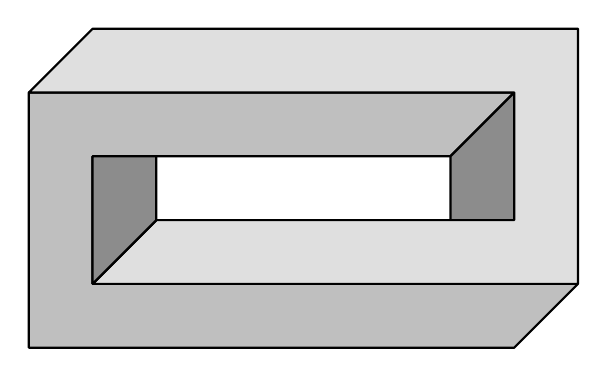
\begin{tikzpicture}[scale=4.5, line join=bevel]
      % \a and \b are two macros defining characteristic
      % dimensions of the impossible brick.
      \pgfmathsetmacro{\a}{0.18}
      \pgfmathsetmacro{\b}{1.37}

      \tikzset{%
        apply style/.code={\tikzset{#1}},
        brick_edges/.style={thick,draw=black},
        face_colourA/.style={fill=gray!50},
        face_colourB/.style={fill=gray!25},
        face_colourC/.style={fill=gray!90},
      }

      \foreach \theta/\v/\facestyleone/\facestyletwo in {%
        0/0/{brick_edges,face_colourA}/{brick_edges,face_colourC},
        180/-\a/{brick_edges,face_colourB}/{brick_edges,face_colourC}
      }{
      \begin{scope}[rotate=\theta,shift={(\v,0)}]
        \draw[apply style/.expand once=\facestyleone]  		
          ({-.5*\b},{1.5*\a}) --
          ++(\b,0)            --
          ++(-\a,-\a)         --
          ++({-\b+2*\a},0)    --
          ++(0,-{2*\a})       --
          ++(\b,0)            --
          ++(-\a,-\a)         --
          ++(-\b,0)           --
          cycle;
        \draw[apply style/.expand once=\facestyletwo] 
          ({.5*\b},{1.5*\a})  --
          ++(0,{-2*\a})       --
          ++(-\a,0)           --
          ++(0,\a)            --
          cycle;
        \end{scope}
      }
    \end{tikzpicture}



See Listing~\ref{lst:autolistingcell116} for the code  display another tikz graphic, as a floating figure.

{

\begin{figure}[tb]
\centering

\begin{normalsize}

\begin{tikzpicture}[font = \sansmath]
  \coordinate (O) at (0,0);

  % ball background color
  \shade[ball color = blue, opacity = 0.2] (0,0) circle [radius = 2cm];

  % cone
  \begin{scope}
    \def\rx{0.71}% horizontal radius of the ellipse
    \def\ry{0.15}% vertical radius of the ellipse
    \def\z{0.725}% distance from center of ellipse to origin

    \path [name path = ellipse]    (0,\z) ellipse ({\rx} and {\ry});
    \path [name path = horizontal] (-\rx,\z-\ry*\ry/\z)
                                -- (\rx,\z-\ry*\ry/\z);
    \path [name intersections = {of = ellipse and horizontal}];

    % radius to base of cone in ball
    \draw[fill = gray!50, gray!50] (intersection-1) -- (0,0)
      -- (intersection-2) -- cycle;
    % base of cone in ball
    \draw[fill = gray!30, densely dashed] (0,\z) ellipse ({\rx} and {\ry});
  \end{scope}

  % label of cone
  \draw (0.25,0.4) -- (0.9,0.1) node at (1.05,0.0) {$q$};

  % ball
  \draw (O) circle [radius=2cm];
  % label of ball center point
  \filldraw (O) circle (1pt) node[below] {$P$};

  % radius
  \draw[densely dashed] (O) to [edge label = $r$] (-1.33,1.33);
  \draw[densely dashed] (O) -- (1.33,1.33);

  % cut of ball surface
  \draw[red] (-1.35,1.47) arc [start angle = 140, end angle = 40,
    x radius = 17.6mm, y radius = 14.75mm];
  \draw[red, densely dashed] (-1.36,1.46) arc [start angle = 170, end angle = 10,
    x radius = 13.8mm, y radius = 3.6mm];
  \draw[red] (-1.29,1.52) arc [start angle=-200, end angle = 20,
    x radius = 13.75mm, y radius = 3.15mm];

  % label of cut of ball surface
  \draw (-1.2,2.2) -- (-0.53,1.83) node at (-1.37,2.37) {$A$};
\end{tikzpicture}
\end{normalsize}
\caption{Caption text for tikz figure\label{fig:tikz-0}}
\end{figure}

}

The next example creates a LaTeX string and outputs it as a Latex object.  The code calculates rules with increasing heights, with this code:


\begin{verbatim}
lstr = '\n\nThis paragraph is embedded as \LaTeX{} in a Jupyter output cell. '\
            + 'One day this could be a complex computed \LaTeX{} string.  '\
            + 'This example only has rising rules...  \n'
for height in range(1,20):
    lstr += '\\rule[0pt]{{10pt}}{}{}pt{} '.format('{',height,'}')
Latex(lstr + '\n')
\end{verbatim}




This paragraph is embedded as \LaTeX{} in a Jupyter output cell. One day this could be a complex computed \LaTeX{} string.  This example only has rising rules...  

\rule[0pt]{10pt}{1pt} \rule[0pt]{10pt}{2pt} \rule[0pt]{10pt}{3pt} \rule[0pt]{10pt}{4pt} \rule[0pt]{10pt}{5pt} \rule[0pt]{10pt}{6pt} \rule[0pt]{10pt}{7pt} \rule[0pt]{10pt}{8pt} \rule[0pt]{10pt}{9pt} \rule[0pt]{10pt}{10pt} \rule[0pt]{10pt}{11pt} \rule[0pt]{10pt}{12pt} \rule[0pt]{10pt}{13pt} \rule[0pt]{10pt}{14pt} \rule[0pt]{10pt}{15pt} \rule[0pt]{10pt}{16pt} \rule[0pt]{10pt}{17pt} \rule[0pt]{10pt}{18pt} \rule[0pt]{10pt}{19pt} 

Jelte Fennema wrote pylatex\cite{httpsgithubcomJelteF00002} to create LaTeX text using Python code.  He wrote the code to create complete documents, but also to write  fragments\cite{httpsjeltefgithubioP00003} --- which we can use here: "Classes can be part of a single document, or can act as pieces on their own. With the \verb+dumps\_as\_content+ method, most classes can return their LaTeX-formatted code, and with the \verb+generate\_tex+ method, this code can be written to a file."


I only spent limited time on pylatex and got the following example to work (it requires \verb+pip install pylatex+).




See Listing~\ref{lst:autolistingcell120} for the code  to format a numy array in \LaTeX{}.

\[%
arr= \begin{bmatrix}%
0.8058753550783919&-0.9307157407593222&-0.5730384566704769&-1.0031754921691696\\%
0.3047454620713325&0.7856317228477806&0.6129561965442012&-0.17388707255129718\\%
-0.8692311208201989&-0.4492042690476358&-0.6185837790516014&0.07556440398337647\\%
0.6039554810033699&-0.27574851788047&0.7335459778270681&1.3255372832207066\\%
-0.7616533999948819&0.7898604029456375&0.2644837689705788&-1.2556993688038824\\%
-0.07910062888605655&-0.9321034462016763&0.8348238145374864&-0.41238021318098034%
\end{bmatrix}%
\]

\chapter{Math}
\label{sec:Math}

Inline math delineated with single dollar symbols are rendered inline with paragraph text, as in $\alpha+\beta=\gamma$.


Using math mode (anything between two dollar symbols) is interpreted as \LaTeX{} math:


\begin{equation}D_{KL}(P||Q) = \sum\limits_{i}ln (\frac{P(i)}{Q(i)}) P(i).\end{equation}


\begin{equation}\begin{array}{llll}E = \frac{\phi}{A_o} = \int \left[\right.&&&\\&\tau_a(R) \tau_o &&\\&\left[\right.&&\\&&\mkern-82mu \Omega_t k_i\left(\epsilon_t L(T_t)\right)&[1]\\&&\mkern-99mu +\,\,\Omega_t k_i(1-\epsilon_t)\left(\frac{\rho E_\textrm{sun}}{\pi}\right)&[2]\\&&\mkern-98mu +\,\,\Omega_t(1-k_i)(1-\epsilon_t)\left(\frac{\rho E_\textrm{sun}}{\pi}\right)&[3]\\&&\mkern-98mu  +\,\, (\Omega_p -\Omega_t) \left(\frac{\rho E_\textrm{sun}}{\pi}\right)&[4]\\&\left.\right]&&\\&+\,\,\tau_o L_\textrm{path}(R) \Omega_p&&[5]\\&\left.\right]d\lambda& &\end{array}\end{equation}


The probability density function for yaw angle is the wrapped normal distribution\cite{httpsenwikipediaorgw00004}.  The first form uses two dollar symbols  to show the equation in LaTeX display math:


\begin{equation}f_{WN}(\theta;\mu, \sigma) = \frac{1}{\sigma\sqrt{2\pi}}\sum^{\infty}_{k=-\infty} \exp\left[\frac{-(\theta-\mu+2\pi k)^2}{2\sigma^2}\right]\end{equation}


The second example uses  \verb+begin{equation}+ and \verb+end{equation}+:


\begin{equation}f_{WN}(\theta;\mu, \sigma) = \frac{1}{\sigma\sqrt{2\pi}}\sum^{\infty}_{k=-\infty} \exp\left[\frac{-(\theta-\mu+2\pi k)^2}{2\sigma^2}\right]\end{equation}


\begin{equation}\begin{array}{l}X_{WN}(\theta;\mu, \sigma) = \frac{1}{\sigma\sqrt{2\pi}}\sum^{\infty}_{k=-\infty} \exp\left[\frac{-(\theta-\mu+2\pi k)^2}{2\sigma^2}\right]\end{array}\end{equation}



\section{Known deficiencies}
\label{sec:Knowndeficiencies}

\begin{enumerate}
\item Some complex cell-merged HTML tables may not render correctly in LaTeX (let me know if you have such a table).
\item Unicode not yet handled.
\item The following HTML elements are not currently processed, these elements are simply ignored: \verb+div+, \verb+iframe+, \verb+img+.
\item Many reserved LaTeX symbols such as hash, caret, underscore and dollar are 'legal' in normal markdown.  When rendering to LaTeX these symbols cause errors unless escaped with backslash.  In many cases these symbols are escaped, but not always because of context.  If the symbols are escaped, they render incorrectly in normal Markdown. Therefore, choose your target renderer and enter the symbols accordingly, accepting problems in the alternative renderer.
\item IPython notebook names must not have spaces in the filename.
\end{enumerate}


\section{Python and module versions, and dates}
\label{sec:Pythonandmoduleversionsanddates}



See Listing~\ref{lst:autolistingcell129} for the code  to get software versions.


\begin{lstlisting}[style=outcellstyle]
Python implementation: CPython
Python version       : 3.8.3
IPython version      : 7.19.0

numpy : 1.19.2
scipy : 1.5.2
pyradi: 1.1.2

Compiler    : MSC v.1916 64 bit (AMD64)
OS          : Windows
Release     : 10
Machine     : AMD64
Processor   : Intel64 Family 6 Model 165 Stepping 2, GenuineIntel
CPU cores   : 16
Architecture: 64bit

Git hash: e4b6b0777ebda4b2ed7d5f3a4130ac58adf56499


\end{lstlisting}



\chapter{Listings}


\begin{lstlisting}[style=incellstyle,caption={Code Listing in cell 58}, label=lst:listing1]
# to prepare the environment
from IPython.display import display
from IPython.display import Image
from IPython.display import HTML

import os.path
import numpy as np
%matplotlib inline

import this
\end{lstlisting}


\begin{lstlisting}[style=incellstyle,caption={Code Listing in cell 60}, label=lst:listing2]
#
print(' ')
print('Radius = {}'.format(6))
print('Frontal area = {} m2'.format(7))
print('This is a very long line of python code, that is supposed to flow over to the next line, in order to test the listing display')
\end{lstlisting}


\begin{lstlisting}[style=incellstyle,caption={Code Listing in cell 61}, label=lst:listing3]
# to print the value
a = ['a','b']
for v in a:
    print(v)
\end{lstlisting}


\begin{lstlisting}[style=incellstyle,caption={Code Listing in cell 62}, label=lst:autolistingcell62]
## this should not appear in the body of the doc if float listings
a = [0, 1]
for v in a:
    print(v)
\end{lstlisting}


\begin{lstlisting}[style=incellstyle,caption={Code Listing in cell 64}, label=lst:autolistingcell64]
print('code with no listing caption')
\end{lstlisting}


\begin{lstlisting}[style=incellstyle,caption={Code Listing in cell 66}, label=lst:autolistingcell66]
def doprint(i):
    print('function output {}'.format(i))
    return int(i)
\end{lstlisting}


\begin{lstlisting}[style=incellstyle,caption={Code Listing in cell 67}, label=lst:autolistingcell67]
for i in [1,2,3]:
    si = str(i)
    v = doprint(si)

val = v * 3   
print(val)
print(v)
\end{lstlisting}


\begin{lstlisting}[style=incellstyle,caption={Code Listing in cell 71}, label=lst:figurelisting]
#this figure is given meta data caption parameters, it will be floated in the latex export
display(Image(filename='images/keep-calm-and-code-python_BW.png', width=250, height=250))
print('also force print output')

\end{lstlisting}


\begin{lstlisting}[style=incellstyle,caption={Code Listing in cell 74}, label=lst:autolistingcell74]
#this figure is not given meta data caption parameters, it will be inlined in the latex export
display(Image(filename='images/random-squares-2.png', width=200, height=200))
\end{lstlisting}


\begin{lstlisting}[style=incellstyle,caption={Code Listing in cell 76}, label=lst:autolistingcell76]
%matplotlib inline

import pylab as pl
import numpy as np

t = np.arange(0.0, 2.0, 0.01)
s = np.sin(2*np.pi*t)
pl.plot(t, s)
pl.xlabel('time (s)')
pl.ylabel('voltage (mV)')
pl.title('About as simple as it gets, folks')
pl.grid(True)

\end{lstlisting}


\begin{lstlisting}[style=incellstyle,caption={Code Listing in cell 78}, label=lst:autolistingcell78]
import pyradi.ryplot as ryplot

x = np.linspace(0,10,10)
a = ryplot.Plotter(1,figsize=(3,2))
b = ryplot.Plotter(2,figsize=(3,2))
c = ryplot.Plotter(3,figsize=(3,2))
for i in [1,2]:
    a.plot(1,x,x ** i,'Plotter instance a',label=[str(i)])
    b.plot(1,x,(-x) ** i,'Plotter instance b',label=[str(i)])
    c.plot(1,x,(5-x) ** i,'Plotter instance c',label=[str(i)])
\end{lstlisting}


\begin{lstlisting}[style=incellstyle,caption={Code Listing in cell 81}, label=lst:autolistingcell81]
htmlstr = '<p><img src="images/flow2-zzz.png" width=200 />'
HTML(htmlstr)                 
\end{lstlisting}


\begin{lstlisting}[style=incellstyle,caption={Code Listing in cell 88}, label=lst:autolistingcell88]
# type(eval("this is a test string")) is not list
\end{lstlisting}


\begin{lstlisting}[style=incellstyle,caption={Code Listing in cell 104}, label=lst:autolistingcell104]
import pandas as pd
d = {'one' : pd.Series([1., 2., 3.], index=['a', 'b', 'c']),
     'two' : pd.Series([1., 2., 3., 4.], index=['a', 'b', 'c', 'd'])}

df = pd.DataFrame(d)

HTML(df.to_html())
\end{lstlisting}


\begin{lstlisting}[style=incellstyle,caption={Code Listing in cell 108}, label=lst:autolistingcell108]
# to create the dataframe and write the output to LaTeX object at default font size
import pandas as pd
import numpy as np
from IPython.display import Latex

def makeDateRand(nrows=6, ncols=4):
    dates = pd.date_range('20130101',periods=6)
    df = pd.DataFrame(np.random.randn(nrows,ncols),index=dates,columns=list('ABCD')) 
    return df

df = makeDateRand(nrows=6, ncols=4)
lstr = df.to_latex(column_format='|l|l|p{50mm}|c|r|')
Latex(lstr)


\end{lstlisting}


\begin{lstlisting}[style=incellstyle,caption={Code Listing in cell 109}, label=lst:autolistingcell109]
lstrno = df.to_latex(index=False,column_format='|l|l|p{50mm}|c|r|')
Latex(lstrno)
\end{lstlisting}


\begin{lstlisting}[style=incellstyle,caption={Code Listing in cell 111}, label=lst:autolistingcell111]
# to write the table in LARGE

Latex(lstr)
\end{lstlisting}


\begin{lstlisting}[style=incellstyle,caption={Code Listing in cell 113}, label=lst:autolistingcell113]
# to write a floating table in tiny font size

Latex(lstr)
\end{lstlisting}


\begin{lstlisting}[style=incellstyle,caption={Code Listing in cell 115}, label=lst:autolistingcell115]
# display a tikz graphic
lstr = r"""
    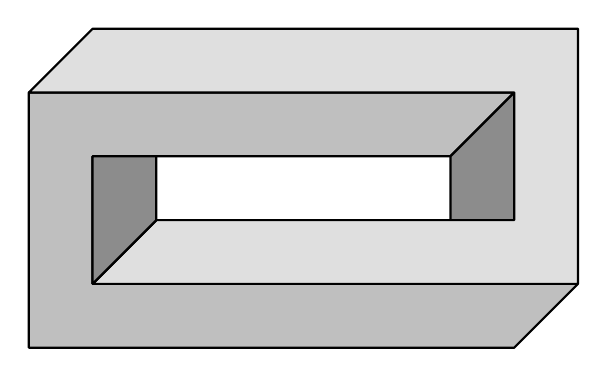
\begin{tikzpicture}[scale=4.5, line join=bevel]
      % \a and \b are two macros defining characteristic
      % dimensions of the impossible brick.
      \pgfmathsetmacro{\a}{0.18}
      \pgfmathsetmacro{\b}{1.37}

      \tikzset{%
        apply style/.code={\tikzset{#1}},
        brick_edges/.style={thick,draw=black},
        face_colourA/.style={fill=gray!50},
        face_colourB/.style={fill=gray!25},
        face_colourC/.style={fill=gray!90},
      }

      \foreach \theta/\v/\facestyleone/\facestyletwo in {%
        0/0/{brick_edges,face_colourA}/{brick_edges,face_colourC},
        180/-\a/{brick_edges,face_colourB}/{brick_edges,face_colourC}
      }{
      \begin{scope}[rotate=\theta,shift={(\v,0)}]
        \draw[apply style/.expand once=\facestyleone]  		
          ({-.5*\b},{1.5*\a}) --
          ++(\b,0)            --
          ++(-\a,-\a)         --
          ++({-\b+2*\a},0)    --
          ++(0,-{2*\a})       --
          ++(\b,0)            --
          ++(-\a,-\a)         --
          ++(-\b,0)           --
          cycle;
        \draw[apply style/.expand once=\facestyletwo] 
          ({.5*\b},{1.5*\a})  --
          ++(0,{-2*\a})       --
          ++(-\a,0)           --
          ++(0,\a)            --
          cycle;
        \end{scope}
      }
    \end{tikzpicture}
"""

Latex(lstr)
\end{lstlisting}


\begin{lstlisting}[style=incellstyle,caption={Code Listing in cell 116}, label=lst:autolistingcell116]
# display another tikz graphic, as a floating figure

lstr = r"""
\begin{tikzpicture}[font = \sansmath]
  \coordinate (O) at (0,0);

  % ball background color
  \shade[ball color = blue, opacity = 0.2] (0,0) circle [radius = 2cm];

  % cone
  \begin{scope}
    \def\rx{0.71}% horizontal radius of the ellipse
    \def\ry{0.15}% vertical radius of the ellipse
    \def\z{0.725}% distance from center of ellipse to origin

    \path [name path = ellipse]    (0,\z) ellipse ({\rx} and {\ry});
    \path [name path = horizontal] (-\rx,\z-\ry*\ry/\z)
                                -- (\rx,\z-\ry*\ry/\z);
    \path [name intersections = {of = ellipse and horizontal}];

    % radius to base of cone in ball
    \draw[fill = gray!50, gray!50] (intersection-1) -- (0,0)
      -- (intersection-2) -- cycle;
    % base of cone in ball
    \draw[fill = gray!30, densely dashed] (0,\z) ellipse ({\rx} and {\ry});
  \end{scope}

  % label of cone
  \draw (0.25,0.4) -- (0.9,0.1) node at (1.05,0.0) {$q$};

  % ball
  \draw (O) circle [radius=2cm];
  % label of ball center point
  \filldraw (O) circle (1pt) node[below] {$P$};

  % radius
  \draw[densely dashed] (O) to [edge label = $r$] (-1.33,1.33);
  \draw[densely dashed] (O) -- (1.33,1.33);

  % cut of ball surface
  \draw[red] (-1.35,1.47) arc [start angle = 140, end angle = 40,
    x radius = 17.6mm, y radius = 14.75mm];
  \draw[red, densely dashed] (-1.36,1.46) arc [start angle = 170, end angle = 10,
    x radius = 13.8mm, y radius = 3.6mm];
  \draw[red] (-1.29,1.52) arc [start angle=-200, end angle = 20,
    x radius = 13.75mm, y radius = 3.15mm];

  % label of cut of ball surface
  \draw (-1.2,2.2) -- (-0.53,1.83) node at (-1.37,2.37) {$A$};
\end{tikzpicture}
"""

Latex(lstr)
\end{lstlisting}


\begin{lstlisting}[style=incellstyle,caption={Code Listing in cell 118}, label=lst:autolistingcell118]
##
lstr = '\n\nThis paragraph is embedded as \LaTeX{} in a Jupyter output cell. '\
            + 'One day this could be a complex computed \LaTeX{} string.  '\
            + 'This example only has rising rules...  \n\n'
for height in range(1,20):
    lstr += '\\rule[0pt]{{10pt}}{}{}pt{} '.format('{',height,'}')
Latex(lstr + '\n')
\end{lstlisting}


\begin{lstlisting}[style=incellstyle,caption={Code Listing in cell 120}, label=lst:autolistingcell120]
# to format a numy array in \LaTeX{}
import numpy as np
# install with pip install pylatex
import pylatex as pyl

arr = makeDateRand(nrows=6, ncols=4).values
matrix = pyl.Matrix(arr, mtype='b')
math = pyl.Math(data=['arr=', matrix])
Latex(math.dumps_as_content())   

\end{lstlisting}


\begin{lstlisting}[style=incellstyle,caption={Code Listing in cell 129}, label=lst:autolistingcell129]
# to get software versions
# https://github.com/rasbt/watermark
# you only need to do this once
# pip install watermark

%load_ext watermark
%watermark -v -m -p numpy,scipy,pyradi -g 
\end{lstlisting}


\begin{lstlisting}[style=incellstyle,caption={Code Listing in cell 130}, label=lst:autolistingcell130]

\end{lstlisting}



\bibliographystyle{IEEEtran}
\bibliography{test2LaTeX}

\end{document}

